Graph theory is the branch of mathematics that studies pairwise
relations between objects. Graphs both appear as tools for analyzing
issues in \ac{HPC}, and as objects of study themselves. This
appendix introduces the basic concepts and some relevant theory.

\Level 0 {Definitions}

A graph consists of a set of objects, and set of relations between them.
The objects, called the \indexterm{nodes}
or \indexterm{vertices} of the graph, usually form a finite set, so we
usually identify them with consecutive integers $1\ldots n$ or $0\ldots
n-1$. The relation that holds between nodes is described by the
\indexterm{edges} of the graph: if $i$ and~$j$ are related, we say
that $( i,j)$ is an edge of the graph. This relation does not need to
be symmetric, take for instance the `less than' relation.

Formally, then, a graph is a tuple $G=\langle V,E\rangle$ where
$V=\{1,\ldots n\}$ for some~$n$, and $E\subset\{(i,j)\colon 1\leq
i,j\leq n,\,i\not=j\}$.

\begin{figure}[ht]
  \hbox{$\vcenter{\hbox{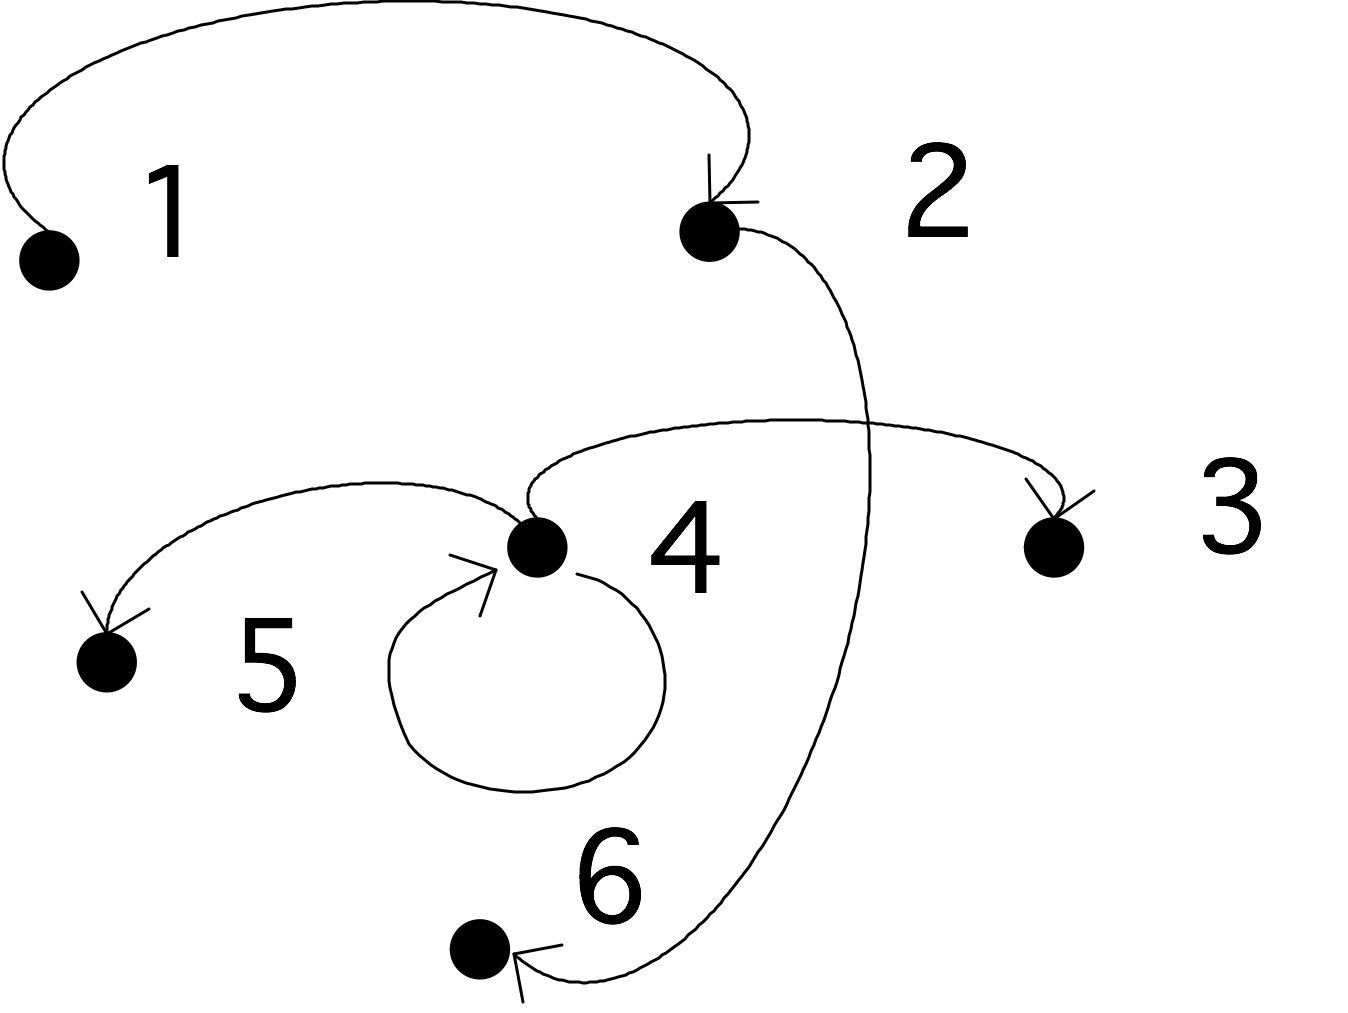
\includegraphics[scale=.1]{graphics/graph1}}}$
    $
    \begin{cases}
      V=\{1,2,3,4,5,6\}\\
      E=\{ (1,2),(2,6),(4,3),(4,4),(4,5)\}
    \end{cases}
    $}
  \caption{A simple graph}
  \label{fig:graph1}  
\end{figure}

A graph is called an \indextermsub{undirected}{graph} if $(i,j)\in
E\Leftrightarrow (j,i)\in E$. The alternative is a
\indextermsub{directed}{graph}, where we indicate an edge $(i,j)$ with
an arrow from $i$ to~$j$.

Two concepts that often appear in graph theory are the
degree and the diameter of a graph. 

\begin{definition}
The
\indexterm{degree} denotes the maximum number of nodes that are
connected to any node:
\[ 
  d(G)\equiv \max_i 
  \left|\{j\colon j\not=i\wedge (i,j)\in E\}\right|.
\]
\end{definition}

\begin{definition}
The \indexterm{diameter} of a graph is the length of the longest
shortest path
in the graph, where a \emph{path}\index{path (graph theory)}
is defined as a set of vertices
$v_1,\ldots, v_{k+1}$ such that $v_i\not=v_j$ for all $i\not=j$ and
\[ \forall_{1\leq i\leq k}\colon (v_i,v_{i+1})\in E. \]
The length of this path is~$k$.
\end{definition}
The concept of diameter is illustrated
in figure~\ref{fig:graph2}.

\begin{figure}[ht]
  \hbox{$\vcenter{\hbox{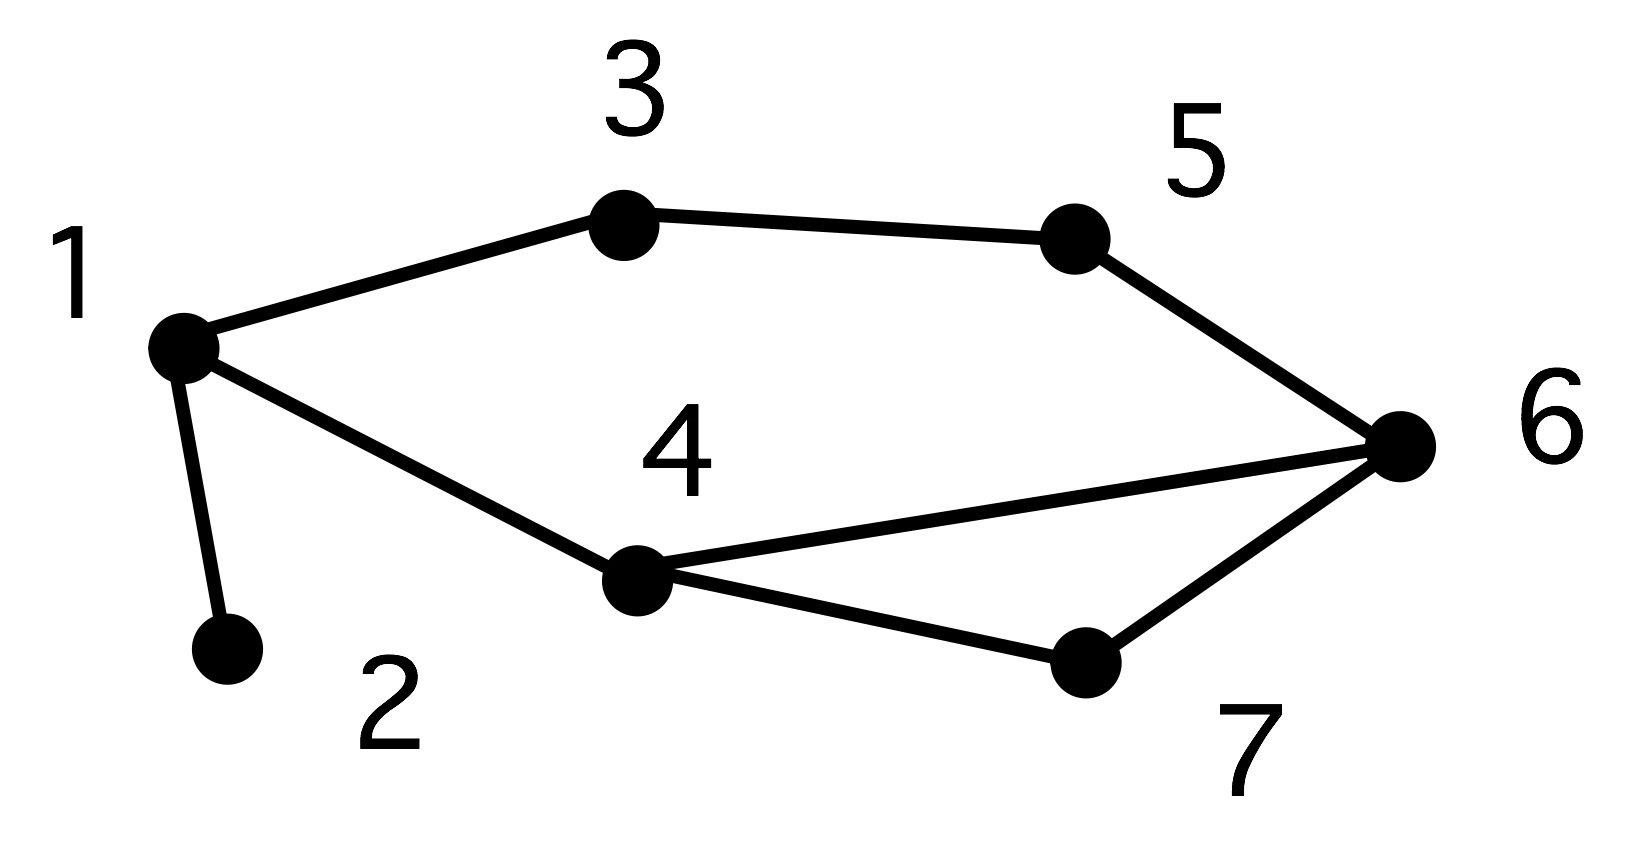
\includegraphics[scale=.1]{graphics/graph2a}}}$
    A graph}
  \hbox{$\vcenter{\hbox{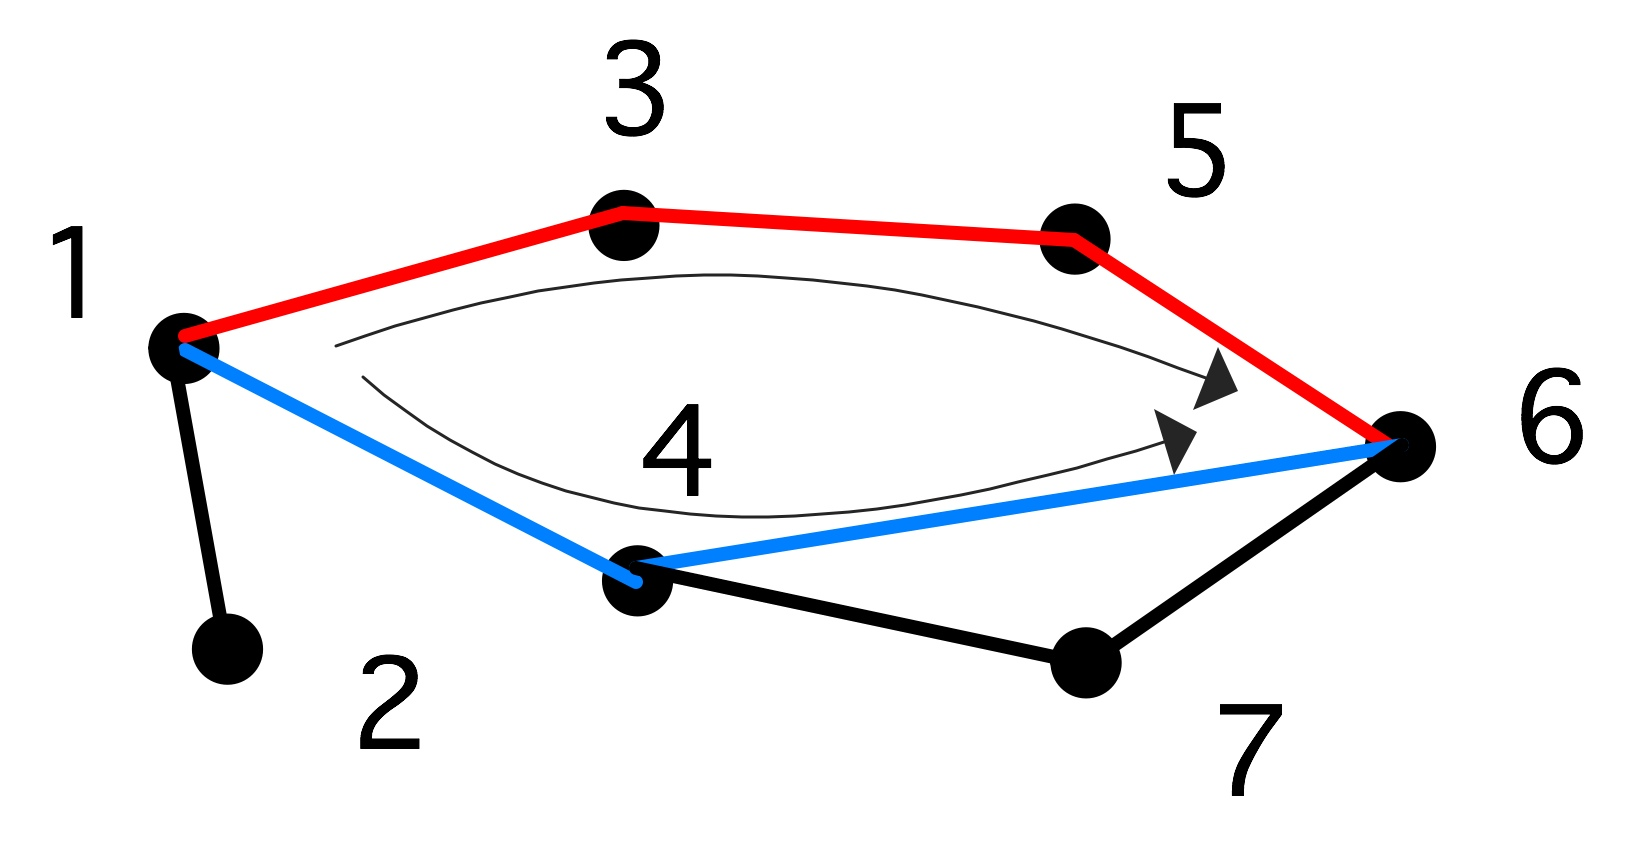
\includegraphics[scale=.1]{graphics/graph2b}}}$
    Two paths from 1 to 6; $\langle 1,4,6\rangle$ is the shorter}
  \hbox{$\vcenter{\hbox{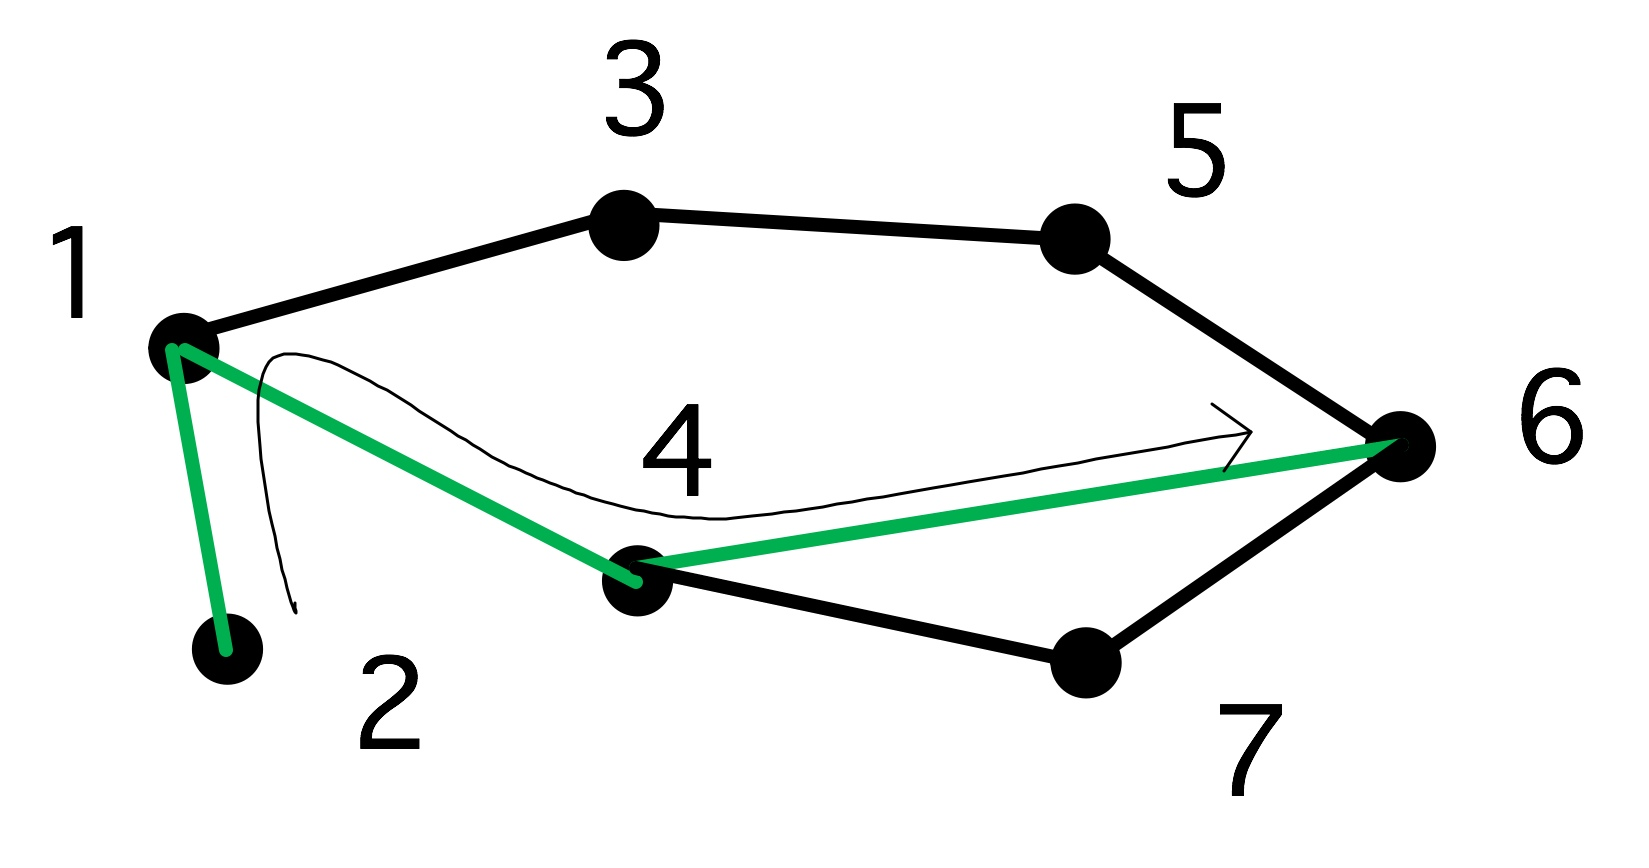
\includegraphics[scale=.1]{graphics/graph2c}}}$
    The longest shortest path of this graph}
  \caption{Shortest paths}
  \label{fig:graph2}
\end{figure}

A~path where all nodes are disjoint
except for $v_1=v_{k+1}$ is called a \emph{cycle}\index{cycle (in graph)}.

Sometimes we are only interested in the mere existence of an edge
$(i,j)$, at other times we attach a value or `weight' $w_{ij}$ to that
edge. A~graph with weighted edges is called a \indexterm{weighted
  graph}. Such a graph can be represented as a tuple $G=\langle
V,E,W\rangle$ where $E$ and $W$ have the same cardinality.

\Level 0 {Common types of graphs}

\Level 1 {Directed Acyclic Graphs}

A graph that does not have cycles is called
\emph{acyclic}\index{acyclic graph}. A special case of this type of
graph is the \indexacf{DAG}. This type of graph can for instance be
used to model dependencies between tasks: if there is an edge between
$i,j$, it means that task $i$ has to be done before task~$j$.

\Level 1 {Trees}

One special case of \acp{DAG} is the \indexterm{tree graph}: here any
node can have multiple incoming edges, but only one outgoing
edge. Nodes with no incoming edges are \indexterm{leaf nodes}; a node
with no outgoing edges is called a root (can there be more than one
root?), and all other nodes are called \indexterm{interior nodes}.

\Level 0 {Graph colouring and independent sets}
\label{sec:independent}
\index{graph!colouring|(}

We can assign labels to the nodes of a graph, which is equivalent to
partitioning the set of nodes into disjoint subsets. One type of
labeling that is of interest is \emph{graph colouring}: here the
labels (or `colours') are chosen so that, if nodes $i$ and~$j$ have
the same colour, there is no edge connecting them: $(i,j)\not\in
E$. 

There is a trivial colouring of a graph, where each node has its own
colour. More interestingly,
the minimum number of colours with which you can colour a graph is
called the \indexterm{colour number} of the graph.

\begin{exercise}
  Show that, if a graph has degree~$d$, the colour number is at
  most~$d+1$.
\end{exercise}

A~famous graph colouring problem is the `four colour theorem': if
a graph depicts countries on a two-dimensional map (a so-called
`planar' graph), then the colour number is at most four.
In general, finding the colour number is hard (in fact, NP-hard).

The colour sets of a graph colouring are also called
\indexterm{independent sets}, since within each colour no node is
connected to a node of the same colour.

There is a trivial way of finding independent sets: declare each node
to have its own unique colour. On the other hand, finding the `best'
division in independent sets, for instance through finding the colour
number of the graph, is difficult. However, often it is enough to find
a reasonable partitioning of the nodes into independent sets, for
instance in constructing paralell ILU preconditioners;
section~\ref{sec:parallel-ilu}. The following algorithm does
that~\cite{jopl94,Luby:parallel}:
\begin{itemize}
\item Give each node a unique random number.
\item Now find the set of nodes that have a higher number than all of
  their neighbours; call this the first independent set.
\item Remove this set from the graph, and find again the nodes with a
  higher number than all their neighbours; this will be the second
  set.
\item Repeat this procedure until all nodes are in an independent set.
\end{itemize}
\begin{exercise}
  Convince yourself that the sets found this way are indeed independent.
\end{exercise}

\index{graph!colouring|)}

\Level 0 {Graphs and matrices}
\index{matrix!adjacency@see{adjacency matrix}}
\index{graph!adjacency@see{adjacency graph}}

A graph can be rendered in a number of ways. You could of course just
list nodes and edges, but little insight can be derived that way.
Simple graphs can be  visualized by drawing vertices and edges, but
for large graphs this becomes unwieldy. Another option is to construct
the \indexterm{adjacency matrix} of the graph. For a graph $G=\langle
V,E\rangle$, the adjacency matrix $M$ (with a size $n$ equal to the
number of vertices~$|V|$) is defined by
\[ 
  M_{ij}=
  \begin{cases}1&(i,j)\in E\\ 0&\mbox{otherwise}\end{cases}
\]
Conversely, if you have a matrix, especially a
\indextermbus{sparse}{matrix}, you can construct its
\indexterm{adjacency graph}.
This is illustrated in figure~\ref{fig:matrix-graph} for
\begin{figure}[ht]
  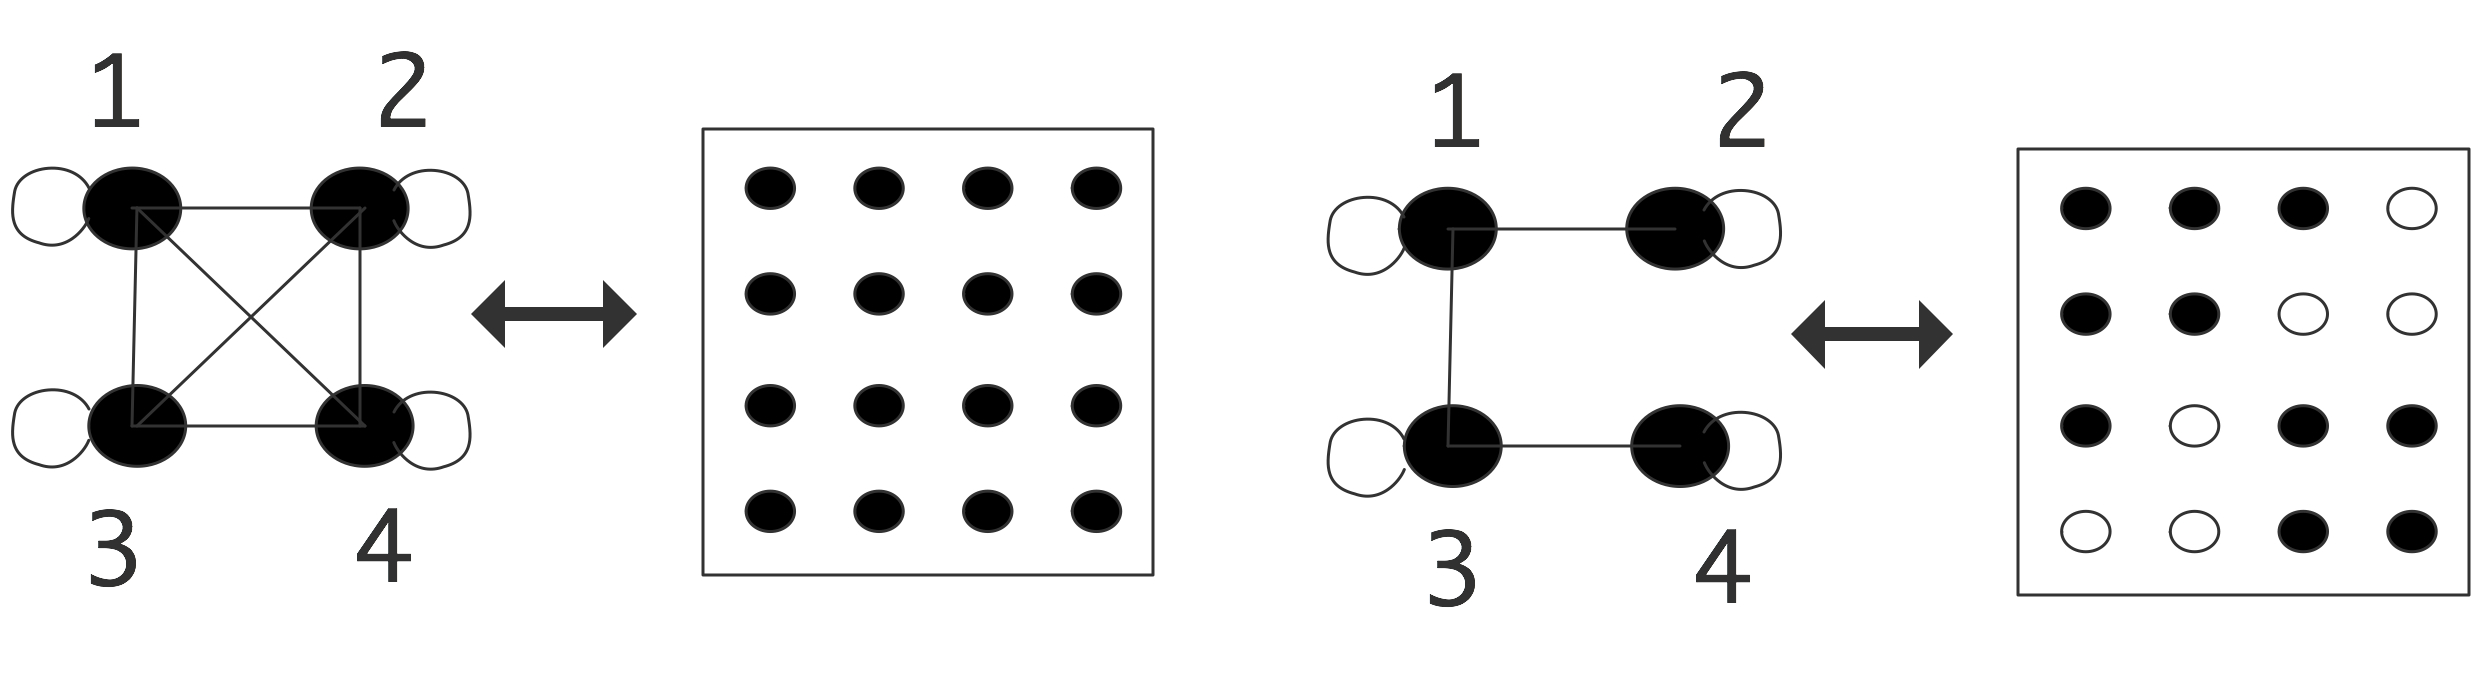
\includegraphics[scale=.14]{graphics/matrix-graph}
  \caption{A dense and a sparse matrix, both with their adjacency
    graph}
  \label{fig:matrix-graph}
\end{figure}
both a dense and a sparse matrix. In this example, the matrices are
structurally symmetric, so we use lines instead of arrows in the
graphs. There is an edge on each vertex corresponding to the diagonal
element; this edge will often be left out of illustrations.

If a matrix has no zero elements, its adjacency graph has an edge
between each pair of vertices. Such a graph is called a
\indexterm{clique}.
If the graph is undirected, the adjacency matrix is symmetric, and
conversely, if a matrix is \indexterm{structurally symmetric}, its
adjacency graph is undirected.

As an example of graph concepts that can easily be read from the
adjacency matrix, consider reducibility.

\begin{definition}
A graph is called \indexterm{irreducible} if for every pair $i,j$ of
nodes there is a path from $i$ to~$j$ and from $j$ to~$i$. A~graph is
reducible if it is not irreducible.
\end{definition}

\begin{exercise}
  Let $A$ be a matrix
  \[ A=
  \begin{pmatrix}
    B&C\\ \emptyset&D
  \end{pmatrix}
  \]
  where $B$ and $D$ are square matrices. Prove the reducibility of the
  graph of which this is the adjacency matrix.
\end{exercise}

For graphs with edge weights, we set the elements of the adjacency
matrix to the weights:
\[ 
  M_{ij}=
  \begin{cases}w_{ij}&(i,j)\in E\\ 0&\mbox{otherwise}\end{cases}
\]
Here is another example of how adjacency matrices can simplify
reasoning about graphs.
\begin{exercise}
  Let $G=\langle V,E\rangle$ be an undirected graph, and let $G'=\langle
  V,E'\rangle$ be the graph with the same vertices, but with vertices
  defined by
  \[ (i,j)\in E'\Leftrightarrow \exists_k\colon (i,k)\in E\wedge
  (k,j)\in E. \]
  If $M$ is the adjacency matrix of~$G$, show that $M^2$ is the
  adjacency matrix of~$G'$, where we use boolean multiplication on the
  elements: $1\cdot1=1$, $1+1=1$.
\end{exercise}

\Level 0 {Spectral graph theory}
\label{app:fiedler}

With a graph $G$ and its adjacency matrix~$A_G$, we can define a
\indexterm{stochastic matrix} or \indexterm{Markov matrix} by scaling
$A_G$ to have unit column sums\footnote{A~definition using unit row
  sums is possible too, in that case every product $Ax$ appearing in
  algorithms is replaced by $x^tA$.}:
\[ W_G = D_G\inv A_G\qquad \hbox{where $(D_G)_{ii}=\deg(i)$}. \]
This matrix describes random walks through the graph. Interpret the
vertices of the graph as locations or states, meaning you can be in
exactly one of them at any time. Let a vector
$p$ be a description of the 
probabilities of being in the nodes of~$G$, then $e^tp=1$.
Now we interpret the edge weights as the probabilities of making a
transition to another node. Mathematically,
$tW_Gp$ describes the probabilities after a single transition. Note
that normalizing the column sums means that these transition
probabilities add up to~1.

Another matrix to associate with a graph is the
\indextermbus{graph}{Laplacian}
\[ L_G = D_G-A_G. \]
This matrix has zero rowsums and positive diagonal entries, so by the
Gershgorin theorem (section~\ref{app:gershgorin} all its eigenvalues
are in the complex right half plane. 

\begin{exercise}
  Show that the vector of all ones is an eigenvector with eigenvalue~1.
\end{exercise}

This Laplacian matrix gives us a quadratic form:
\[ x^tL_Gx = \sum_{(i,j)\in E} (x_i-x_j)^2. \]

\Level 1 {Eigenvalue theorems for graph matrices}
\label{sec:fiedler-vector}

There are various interesting theorems connected with the graph
adjacency and Laplacian matrix. We will not give any proofs;
see~\cite{Spielman:spectral-graph-theory}.

First we give \indexterm{Fiedler's theorem}.
\begin{theorem}
  Let $G$ be a weighted path graph on $n$ vertices, let $L_P$ have
  eigenvalues $0 = \lambda_1 < \lambda_2\leq\ldots\leq\lambda_n$, and let
  $v_k$ be an eigenvector of~$\lambda_k$. Then $v_k$ changes sign
  $k-1$ times.
\end{theorem}

Another theorem by Fiedler~\cite{Fiedler:75-property}:
\begin{theorem}
  Let $G = (V,E,w)$ be a weighted connected graph, and let $L_G$ be
  its Laplacian matrix. Let $0 = \lambda_1 < \lambda_2 \leq \cdots
  \leq \lambda_n$ be the eigenvalues of $L_G$ and let $v_1,\ldots,v_n$
  be the corresponding eigenvectors. For any $k \geq 2$, let $W_k
  =\{i\in V\colon v_k(i)\geq0\}$. Then, the graph induced by $G$ on $W_k$
  has at most $k-1$ connected components.
\end{theorem}

The important consequence of this is that the eigenvector to the first
nontrivial eigenvalue can be used to partition the graph in two connected
pieces: one of nodes where the eigenvector is positive, and one where
the eigenvector is negative.

The adjacency matrix is nonnegative, and there is an extensive theory
for this type of matrix~\cite{BePl:book}; see the Perron-Frobenius
theorem in section~\ref{app:perron}.

\begin{lemma}
  The largest eigenvalue of the adjacency matrix can be bounded by the
  maximum node degree:
  \[ \alpha_1\leq d_{\max}. \]
\end{lemma}

\Level 1 {Cheeger's inequality}

Above we remarked that the first non-trivial eigenvalue of the graph
Laplacian has a relation to partitioning a graph in two parts. The
\indextermbus{Cheeger's}{constant} and
\indextermbus{Cheeger's}{inequality} relate this eigenvalue to a
certain quality measure of partitionings.

Let $V$ be the set of vertices and $S\subset V$, then Cheeger's
constant of a graph is defined as
\[ C=\min_S \frac{e(S,V-S)}
        {\min{\mathord{\mathrm{vol}}(S),\mathord{\mathrm{vol}}(V-S)}}
\]
where $e(S,V-S)$ denotes the number of edges connecting $S$ to $V-S$,
and the volume of a set of nodes is defined as
\[ \mathord{\mathrm{vol}}(S) = \sum_{e\in S}d(e). \]

Cheeger's inequality then states
\[ 2C \geq \lambda \geq \frac{C^2}2 \]
where $\lambda$ is the first nontrivial eigenvalue of the graph
Laplacian.
